%%
%%  Example paper
%%
%%

%%%%%%%%%%%%%%%%%% Usenix style %%%%%%%%%%%%%%%%%%%%%%%%%%%%%%%%%
\documentclass[10pt,twocolumn,a4paper]{article}
\usepackage{styles/usenix-style}

\author{Put your name here}

%%%%%%%%%%%%%%%%%% Document %%%%%%%%%%%%%%%%%%%%%%%%%%%%%%%%%%%%%%%%%%%
% TODO: Change draft to final before submitting final version.
\usepackage[draft]{styles/ka-style}
\usepackage{cite,xspace,ifthen,graphicx,listings}

\usepackage[
   pdfauthor={Author},
   pdftitle={A Paper Template},
   pdfsubject={Paper Template},
   pdfkeywords={Papers, Templates}
]{hyperref}

\begin{document}

\title{ Put the title of your seminar report here }

\newcommand{\todo}[1]{{\texttt{[#1]}}}
\newcommand{\code}[1]{{\tt \small{#1}}}

\maketitle
%\draftfooter

\begin{abstract}
Bla.
\end{abstract}

\section{Introduction}\label{sec:introduction}
\section{Background}\label{sec:background}

\begin{figure}[htbp]
  \centering
  \fbox{\parbox{.8\columnwidth}{
      Here you can include a sample figure.  Use something like
      \begin{center}
        \code{$\backslash$includegraphics[scale=.8]\{template\}}
      \end{center}
      to include an encapsulated postscript figure.  The \emph{scale}
      argument can be used for scaling the picture, although it
      may scale the font incorrectly.
    }}
  \caption{Sample Figure}
  \label{fig:sample}
\end{figure}


\lstset{language=C, basicstyle=\ttfamily,
        string=[b]', showspaces=false, showtabs=false,
        caption={A sample code snippet}, captionpos=b}
\begin{lstlisting}
/* code snippet  */
while (!sleep)
	sleep++;
\end{lstlisting}

\begin{figure}[hbt]
\centering
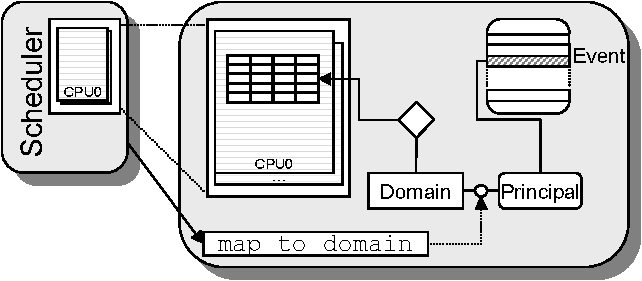
\includegraphics[scale=.7,clip]{fig/template}
\caption{Sample figure automatically from Windows prn.\label{plot:fig}}
\end{figure}

\section{Related Work}\label{sec:relwork} 

Works \cite{xen03virtualization} and \cite{pratt2005xaa} are relevant but
different.

\section{Approach}

\section{Conclusion}\label{sec:conclusion}

\bibliographystyle{abbrv}
\bibliography{template}
%\footnotesize
\end{document}
